% Phylogenetic tree with 3 leaves (from the phylo-icms paper, Fig. 1 left).
\tikzset{every picture/.style={line width=0.9pt}}
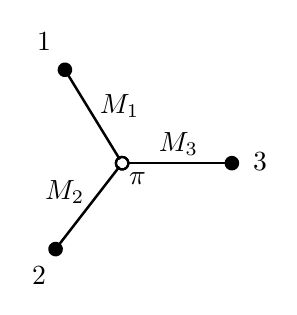
\begin{tikzpicture}[x=0.75pt,y=0.75pt,yscale=-0.9,xscale=0.9]
%Straight Lines [id:da6480600435039572]
\draw    (-7.73,75.65) -- (21.67,123.65) ;
\draw [shift={(22.9,125.65)}, rotate = 58.51] [color={rgb, 255:red, 0; green, 0; blue, 0 }  ][line width=0.75]      (0, 0) circle [x radius= 3.35, y radius= 3.35]   ;
\draw [shift={(-7.73,75.65)}, rotate = 58.51] [color={rgb, 255:red, 0; green, 0; blue, 0 }  ][fill={rgb, 255:red, 0; green, 0; blue, 0 }  ][line width=0.75]      (0, 0) circle [x radius= 3.35, y radius= 3.35]   ;
%Straight Lines [id:da5995917630568086]
\draw    (21.46,127.51) -- (-12.73,171.65) ;
\draw [shift={(-12.73,171.65)}, rotate = 127.76] [color={rgb, 255:red, 0; green, 0; blue, 0 }  ][fill={rgb, 255:red, 0; green, 0; blue, 0 }  ][line width=0.75]      (0, 0) circle [x radius= 3.35, y radius= 3.35]   ;
\draw [shift={(22.9,125.65)}, rotate = 127.76] [color={rgb, 255:red, 0; green, 0; blue, 0 }  ][line width=0.75]      (0, 0) circle [x radius= 3.35, y radius= 3.35]   ;
%Straight Lines [id:da8445650211886888]
\draw    (25.25,125.65) -- (81.65,125.65) ;
\draw [shift={(81.65,125.65)}, rotate = 0] [color={rgb, 255:red, 0; green, 0; blue, 0 }  ][fill={rgb, 255:red, 0; green, 0; blue, 0 }  ][line width=0.75]      (0, 0) circle [x radius= 3.35, y radius= 3.35]   ;
\draw [shift={(22.9,125.65)}, rotate = 0] [color={rgb, 255:red, 0; green, 0; blue, 0 }  ][line width=0.75]      (0, 0) circle [x radius= 3.35, y radius= 3.35]   ;
% Text Node
\draw (-24.33,53.78) node [anchor=north west][inner sep=0.75pt]  [font=\normalsize]  {$1$};
% Text Node
\draw (-27,179.15) node [anchor=north west][inner sep=0.75pt]  [font=\normalsize]  {$2$};
% Text Node
\draw (91.28,118.14) node [anchor=north west][inner sep=0.75pt]  [font=\normalsize]  {$3$};
% Text Node
\draw (9.27,87.3) node [anchor=north west][inner sep=0.75pt]  [font=\normalsize]  {$M_{1}$};
% Text Node
\draw (-20.12,133.05) node [anchor=north west][inner sep=0.75pt]  [font=\normalsize]  {$M_{2}$};
% Text Node
\draw (40.77,107.3) node [anchor=north west][inner sep=0.75pt]  [font=\normalsize]  {$M_{3}$};
% Text Node
\draw (24.9,129.05) node [anchor=north west][inner sep=0.75pt]  [font=\normalsize]  {$\pi $};
\end{tikzpicture}
